\documentclass{article}

% Langue
\usepackage[utf8]{inputenc}
\usepackage[T1]{fontenc}      
\usepackage[francais]{babel}

% Mise en forme générale
\usepackage[top=2.5cm,bottom=2.5cm,right=2.5cm,left=2.5cm]{geometry}

% Package divers
\usepackage{chemist} 
\usepackage[version=3]{mhchem}
\usepackage{chemfig}
\usepackage[squaren, Gray]{SIunits}
\usepackage{sistyle}
\usepackage[autolanguage]{numprint}
\usepackage{url}
\usepackage{rotating}
\usepackage{xcolor,colortbl}
\definecolor{Gray}{gray}{0.85}

\usepackage{hyperref}
\hypersetup{
    colorlinks,
    citecolor=black,
    filecolor=black,
    linkcolor=black,
    urlcolor=black
}

% Nouvelles commandes
\newcommand{\std}{\ensuremath{^{\circ}}}
\newcommand\ph{\ensuremath{\mathrm{pH}}}
\newcommand{\annexe}{\part{Annexes}\appendix}
\newcommand{\biblio}[1]{\bibliographystyle{plain}\bibliography{#1}\nocite{*}}

\newcommand{\doctitle}[1]{
	\title{#1}
	\author{\textbf{Groupe 124.3}\\
	\textsc{Frenyo} Péter (6266-12-00)\\
	\textsc{Gillain} Nathan (7879-12-00)\\
	\textsc{Lamine} Guillaume (7109-13-00)\\
	\textsc{Piraux} Pauline (2520-13-00)\\
	\textsc{Paris} Antoine (3158-13-00)\\
	\textsc{Quiriny} Simon (4235-13-00)\\
	\textsc{Schrurs} Sébastien (7978-13-00)}
	\date{\today}

	\begin{document}

	\maketitle
	\tableofcontents
}

\usepackage[numbered, framed]{mcode}
\doctitle{Projet 3 - Tache 1}

% ------------------------------------------
% INTRODUCTION
% ------------------------------------------
\section{Introduction}
Afin de fournir des données permettant à notre société Paris © Co. Ltd (Licensed Trademark by Antoine & Bartholomeus Paris) 
d'implanter une usine de production d'ammoniac en Belgique, nous avons réalisé une étude théorique nous fournissant les 
diverses informations nécessaires au bon fonctionnement de notre usine. Celle-ci produit de l'ammoniac à partir de méthane 
via une série de réactions convergeant vers le procédé Haber-Bosch.

Ce rapport fournit premièrement les informations relatives aux réactifs nécessaires à la production d'une quantité fixée 
d'ammoniac, de la quantité d'eau nécessaire au refroidissement permettant d'atteindre la température requise pour que la 
réaction Haber-Bosch ait lieu, la source des réactifs utilisés par la société ainsi que l'énergie nécessaire au réformage 
primaire.

Nous fournissons ensuite un outil de gestion écrit en MATLAB synthétisant les calculs des quantités de matières nécessaires 
à la production d'une masse fixe d'ammoniac à une certaine température du réacteur du réformage primaire. Cet outil fournit 
les valeurs en moles de tout les composés à chaque étape de production.

Nous réalisons ensuite une étude paramétrique permettant la combinaison optimale de température et de production quotidienne 
d'ammoniac correspondant à nos produits disponibles, et nous finissons par un calcul du nombre de tuyaux nécessaires à un 
certain débit de $CH_4$ et de $H_2O$ dans le réformeur primaire.

% ------------------------------------------
% CALCUL DU FLUX DES REACTIFS
% ------------------------------------------
\section{Calcul du flux des réactifs}
\paragraph{Hypothèse}
Lors du calcul de ces flux, nous avons utilisé l'hypothèse que tous les réactifs sont 
consommés par le réacteur.

\paragraph{Calculs}
L'équation de la réaction de production de l'ammoniac par le procédé \textsc{Haber-Bosch} est donnée par :

	\begin{chemmath}
			\frac{1}{2}N_2(g) + \frac{3}{2}H_2(g) \longrightarrow NH_3(g) + \Delta H
 	\end{chemmath}
	
En sachant que l'on cherche à produire \unit{1000}{\ton} de \chemform{NH_3} par jour, 
on calcule assez facilement le flux de \chemform{N_2} (les détails de calculs ont été omis
dans ce rapport)

	$$m_{N_2} = \unit{823.5}{\ton\per\dday}$$

et le flux de \chemform{H_2}

	$$m_{H_2} = \unit{176.4}{\ton\per\dday}.$$

% ------------------------------------------
% CALCUL DU DEBIT D'EAU NECESSAIRE POUR...
% ------------------------------------------
\section{Calcul du débit d'eau nécessaire pour refroidir le réactif}
\paragraph{Hypothèses}
\begin{itemize}
	\item Les capacités calorifiques ne dépendent pas de la température ;
	\item La pression dans le réacteur est constante et vaut \unit{10^5}{\pascal}.
\end{itemize}

\paragraph{Première méthode : on considère les capacités calorifiques constantes}
Pour la réaction donnée dans la section précédente, on a $\Delta H(\unit{298.15}{\kelvin})
 = \unit{-46 \cdot 10^3}{\joule}$ pour une mole de \chemform{NH_3(g)} produite \cite{atkins}.
Comme la réaction a lieu à \unit{500}{\celsius} (c'est à dire \unit{773.15}{\kelvin}), il
va falloir calculer $\Delta H(\unit{773.15}{\kelvin})$. Pour cela, nous avons besoin
des capacités calorifiques moyenne à pression constante de chacun des réactifs et des produits
de la réaction. Nous trouvons ces données dans une table \cite{atkins}.

	$$
	\left\{
		\begin{array}{rl}
			C_{p_{NH_3(g)}} &= \unit{37}{\joule\per\mole\kelvin}\\
			C_{p_{H_2(g)}} 	&= \unit{28.836}{\joule\per\mole\kelvin}\\
			C_{p_{N_2(g)}} 	&= \unit{29.124}{\joule\per\mole\kelvin}
		\end{array}
	\right.
	$$

On a donc :

$$\Delta H(\unit{773.15}{\kelvin}) = \Delta H(\unit{298.15}{\kelvin})
+ \int_{298.15}^{773.15} C_{p_{NH_3(g)}} dT - \frac{1}{2}\int_{298.15}^{773.15} C_{p_{N_2(g)}} dT
- \frac{3}{2} \int_{298.15}^{773.15} C_{p_{H_2(g)}} dT = \unit{-5.5887 \cdot 10^4}{\joule\per\mole}$$

Pour la quantité de \chemform{NH_3} à produire par jour (à savoir $\unit{58.83 \cdot 10^6}{\mole}$),
la quantité de chaleur produite est donc :

$$q = \Delta H(\unit{773.15}{\kelvin}) \cdot n_{NH_3} = \unit{-3.28786 \cdot 10^{12}}{\joule}$$

En connaissant la capacité calorifique de l'eau $C_{H_2O(g)} = \unit{4185.5}{\joule\per\kilo\gram\kelvin}$ \cite{atkins}et en égalant
$q$ à $m_{H_2O} \cdot C_{H_2O(g)} \cdot \Delta T$ avec $\Delta T = 90 - 25 = \unit{65}{\kelvin}$, on trouve un
flux d'eau égal à

$$m_{H_2O} = \unit{1.2085 \cdot 10^7}{\kilo\gram\per\dday} \Rightarrow V_{H_2O} \approx \unit{1.2085 \cdot 10^7}{\liter\per\dday} 
= \unit{139.8}{\liter\per\second}$$

\paragraph{Deuxième méthode : les capacités calorifiques dépendent de la température}
On peut être plus précis en utilisant les capacités calorifiques suivantes \cite{hc-table} :

	$$
	\left\{
		\begin{array}{rl}
			C_{p_{NH_3(g)}}(T) &= \unit{31.81 + (15.48 \cdot 10^{-3})T + (5.86 \cdot 10^{-6})T^2}{\joule\per\mole\kelvin}\\
			C_{p_{H_2(g)}}(T) 	&= \unit{29.30 - (0.84 \cdot 10^{-3})T + (2.09 \cdot 10^{-6})T^2}{\joule\per\mole\kelvin}\\
			C_{p_{N_2(g)}}(T) 	&= \unit{27.62 + (4.19 \cdot 10^{-3})T}{\joule\per\mole\kelvin}
		\end{array}
	\right.
	$$

En refaisant le calcul ci-dessus en tenant compte de la variation des capacités calorifiques en fonction
de la température, nous obtenons un débit un peu inférieur de \unit{135.662}{\liter\per\second}. On remarque
que l'erreur faite en utilisant l'approximation de la section précédente est de 3\%.

% ------------------------------------------
% SOURCES DES REACTIFS
% ------------------------------------------
\section{Sources des réactifs}
	\subsection{Sources de diazote}
	\subsubsection{Procédé cryogénique}
	Ce procédé se base sur la séparation des différents constituants de l'air en fonction de leur température 
	d'ébullition (l'oxygène \chemform{O_2} se condense avant le diazote \chemform{N_2}).
	L'air est purifié jusqu'à liquéfaction et les différents constituants sont séparés dans une colonne de 
	rectification par distillation fractionnée. Cette méthode permet d'avoir du diazote \chemform{N_2} pur 
	à \numprint{99,99}\%. Cette méthode est efficace pour une consommation au-delà de $\unit{200}{\meter\cubed\per\hour}$ \cite{scf}. 

	\subsubsection{Perméation gazeuse}
	Ce procédé utilise les différentes vitesses d'effusion des molécules de gaz à travers une membrane. 
	L'\chemform{O_2}, \chemform{H_2O} et le \chemform{CO_2} s'effusent plus rapidement que le \chemform{N_2}.
	Cette méthode nous permet d'obtenir du \chemform{N_2} sec pur à \numprint{95}-\numprint{99}. Ce procédé s'utilise pour des 
	débits forts variables ($\unit{3-1000}{\meter\cubed\per\hour}$) \cite{scf}.

	\subsubsection{Méthode de Ramsay}
	
	\begin{chemmath}
			NaNO_2(aq) + NH_4Cl(aq) \longrightarrow NaCl(aq) + 2H_2O(l) + N_2(g)
	\end{chemmath}
	
	On chauffe le mélange de \chemform{NaNO_2} et \chemform{NH_4Cl} pour obtenir le \chemform{N_2} sous forme gazeuse.
	Un désavantage de cette méthode par rapport aux 2 premières est qu'il faut acheter les réactifs. De plus, il faut utiliser de l'énergie pour chauffer la réaction \cite{wiki-n2}.

	\subsection{Sources de dihydrogène}
		\subsubsection{Vaporeformage de méthane}
		2 réactions sont utilisées pour ce procédé \cite{afhypac} :
		
		\begin{chemmath} 
			CH_4 + H_2O \longleftrightarrow CO + 3H_2
		\end{chemmath}
		
		\begin{chemmath}
			CO + H_2O \longleftrightarrow CO_2 + H_2
		\end{chemmath}
		
		L'équation bilan obtenue est la suivante :
		
		\begin{chemmath}
			CH_4 + 2H_2O \longleftrightarrow CO_2 + 4 H_2
		\end{chemmath}
		
			Cette réaction nécessite un catalyseur : le nickel. Le rendement varie entre $40-45\%$. Le problème de cette 
			méthode est qu'elle rejette une grande quantité de \chemform{CO_2}, gaz à effet de serre \cite{wiki-h2}.
			
		\subsubsection{Oxydation partielle d'hydrocarbure}
		\begin{chemmath}
			C_nH_m + \frac{n}{2} O_2 + \frac{3,76n}{2} N_2 \longrightarrow \frac{m}{2} H_2 + n CO + \frac{3,76n}{2} N_2
		\end{chemmath}
		L'air est comburant pour cette réaction, qui a besoin d'être catalysée. Son caractère exothermique aide à la catalyse. 
		L'inconvénient de cette méthode est son faible rendement \cite{wiki-h2}.

		\subsubsection{Electrolyse}
		Réaction à l'anode : 
		
		\begin{chemmath}
			2H_2O(l) \longrightarrow O_2(g) + 4 H^+(aq) + 4e^-
		\end{chemmath}
		
		Réaction à la cathode :
		
		\begin{chemmath}
			4H_2O(l) + 4e^- \longrightarrow 2H_2O(g) + 4OH^-(aq)
		\end{chemmath}
		
		L'équation bilan obtenue est la suivante :
		
		\begin{chemmath}
			2H_2O(l) \longrightarrow 2H_2(g) + O_2(g)
		\end{chemmath}
		
	La réaction nécessite une grande quantité d'électricité. L'eau, quant à elle, est présente en quantité illimitée 
	et est peu coûteuse. En pratique, cette méthode est très peu utilisée \cite{wiki-h2}.

% ------------------------------------------
% BILAN DE MATIERE
% ------------------------------------------
\section{Bilan de matiere}
Pour la compréhension de cette section, nous vous renvoyons vers le flow-sheet \ref{appendix:flow-sheet}.
On pose le flux de \chemform{NH_3(g)} à la sortie égal à $\unit{m_{NH_3}}{\gram\per\dday} \footnote{Avec \unit{\gram\per\dday} = grammes par jour.}$. 

Nous utilisons une méthode bottom-up. Nous partons donc de la réaction : 
\begin{chemmath}
		\frac{1}{2}N_2(g) + \frac{3}{2}H_2(g) \longrightarrow NH_3(g) 
\end{chemmath}

Et donc,
 
$$n_{NH_3} = \unit{\frac{m_{NH_3}}{17}}{\mole\per\dday}$$

Ce qui donne les valeurs suivantes pour le nombre de moles final de $N_2$ et de $H_2$ nécessaire ("final" étant donné que, pour rappel, nous partons de la fin) : 

$$n_{N_2f} = \frac{n_{NH_3}}{2} = \unit{\frac{m_{NH_3}}{34}}{\mole\per\dday}$$ 

et 

$$n_{H_2f} = \frac{3}{2} \cdot n_{NH_3}$$

On sait que le \chemform{N_2(g)} provient uniquement de l'air entrant 
dans le réacteur du  réformage primaire. Et comme on a posé comme hypothèse
que l'air est composé de 78\% de \chemform{N_2(g)}, 21\% de \chemform{O_2(g)}
et 1\% d'\chemform{Ar(g)}, on peut déduire que $n_{air}$ entrant dans le 
réacteur du réformage primaire vaut : 

$$n_{air}= n_{N_2} \cdot \frac{100}{78} = \unit{\frac{m_{NH_3}}{26.52}}{\mole\per\dday}$$ 

Et :
$$n_{O_2}= n_{air} \cdot \frac{21}{100} = \unit{\frac{0.21m_{NH_3}}{26.52}}{\mole\per\dday}$$
$$n_{Ar}= n_{air} \cdot \frac{1}{100} = \unit{\frac{0.01m_{NH_3}}{26.52}}{\mole\per\dday}$$

La réaction dans le réformage secondaire, durant laquelle l'air est inséré, est la suivante :
\begin{chemmath}
	2CH_4 + O_2 \Longrightarrow 2CO + 4 H_2
\end{chemmath}  

Nous savons par hypothèse que le
\chemform{CH_4(g)} et le \chemform{O_2(g)} sont présents en quantité stoechiométrique. Nous avons donc la quantité suivante de \chemform{CH_4} à l'entrée du réformage secondaire (rs) : 

$$n_{CH_4rs} = 2 \cdot n_{O_2} = \unit{\frac{0.42m_{NH_3}}{26.52}}{\mole\per\dday}$$
Ainsi que les quantités suivantes de \chemform{CO} et de \chemform{H_2} créés 
$$n_{COrs} = n_{CH_4rs} =  \unit{\frac{0.42m_{NH_3}}{26.52}} {\mole\per\dday}$$
$$n_{H_2rs} = 2 \cdot n_{CH_4rs} =  \unit{\frac{0.84m_{NH_3}}{26.52}}{\mole\per\dday}$$

On s'intéresse ensuite à la réaction du Water-Gas-Shift : 

\begin{chemmath}
	CO + H_2O \Longrightarrow CO_2 + H_2
\end{chemmath} 

% Cette partie n'est pas claire selon la tutrice, à réecrire 
On sait que $n_{COwgs}$  $= n_{COrp}$ 
$+ n_{COrs}$ avec $n_{COwgs}$ le nombre de moles de CO a l'entrée de la réaction Water-Gas-Shift, $n_{COrp}$ celui a la sortie du réformage primaire et $n_{COrs}$ celui à la sortie du réformage secondaire.

Dans la réaction Water-Gas-Shift, nous avons $n_{COwgs}$ moles de CO et un excès de $H_2O$ en réactifs, et $n_{COwgs}$ moles de $CO_2$ et de $H_2$ formés.

$$n_{CO_2} = n_{CO} = n_{H_2}$$

S'il reste du \chemform{H_2O} à la fin de cette réaction, le nombre de moles d'eau à la sortie de la réaction Water-Gas-Shift sera égal aux nombre de moles d'eau à la sortie du réformage primaire moins $n_{COwgs}$ (le nombre de moles utilisés dans la réaction Water-Gas-Shift).
$$n_{H_2O-dégagé} = n_{{H_2Orp}}
- n_{COwgs}$$.

On peut aussi déduire que le nombre de moles de $CO_2$ dégagés à la fin de la réaction Water-Gas-Shift ($n_{CO_2-tot}$) vaut la somme du nombre de moles de $CO_2$ produits par le réformage primaire et par la réaction Water-Gas-Shift : $$n_{CO_2-dégagé} = n_{{CO_2rp}}
+ n_{{CO_2wgs}}$$.

Etant donné que l'on a le nombre de moles de $H_2$ nécessaire à la production de $\unit{m_{NH_3}}{\gram\per\dday}$, qui est de $n_{H_2f}$, et que l'on sait le nombre de moles de $H_2$ produit à travers les diverses réactions, nous savons les égaliser de la manière suivante (les indices "rp", "rs" et "wgs" signifiant "à la \textit{sortie}" du réformage primaire, secondaire et de la réaction Water-Gas-Shift) : 

$$n_{H_2f} = n_{H_2rp} + n_{H_2rs} + n_{H_2wgs}$$

% ------------------------------------------
% EQUILIBRE DU REFORMAGE PRIMAIRE
% ------------------------------------------
\section{Equilibre du reformage primaire}
\subsection{Calcul de la constante d'équilibre}
Pour calculer la constante d'équilibre nous allons utiliser $K= \exp{\frac{-\Delta G}{RT}}$ avec $\Delta G = \Delta H - T\Delta S$.

\subsubsection{Première réaction}
Calculons la constante d'équilibre $K_1$ de la réaction suivante :

\begin{chemmath} 
 CH_4(g) + H_2O(g) \Leftrightarrow CO(g) + 3H_2(g).
\end{chemmath} 

Connaissant l'enthalpie en conditions standards \cite{atkins} et les capacités calorifiques dépendant de la température \cite{hc-table},
$$
\left\{
	\begin{array}{rl}
		C_{p_{CO}}(T) 		&= \unit{27.62 +(5.02 \cdot 10^{-3})T}{\joule\per\mole\kelvin} \\
		C_{p_{H_2}}(T) 		&= \unit{29.3-(0.84 \cdot 10^{-3})T + (2.09\cdot 10^{-6})T^2}{\joule\per\mole\kelvin} \\
		C_{p_{CH_4}}(T) 	&= \unit{14.23+(75.3 \cdot 10^{-3})T - (18\cdot 10^{-6})T^2}{\joule\per\mole\kelvin} \\
		C_{p_{H_2O}}(T) 	&= \unit{30.13+(10.46 \cdot 10^{-3})T}{\joule\per\mole\kelvin} 
	\end{array}
\right.
$$

on peut écrire

$$\Delta C_p(T) = 3C_{p_{H_2}}(T) + C_{p_{CO}}(T) - C_{p_{CH_{4}}}(T) - C_{p_{H_2O}}(T).$$

On peut donc directement calculer $\Delta H_1(T)$ :

$$
	\begin{array}{rl}
		 	 \Delta H_1(T)	= \Delta H(\unit{298.15}{\kelvin}) + \int_{298.15}^T \Delta C_p(T) dT 
											= \unit{188369.87 + 71.16 T -0.04163 T^2 + (8.09\cdot 10^{-6}) T^3}{\joule\per\mole} 
	\end{array}
$$	

Connaissant l'entropie en conditions standards \cite{atkins}, on peut 
également directement calculer $\Delta S_1$
 
$$
	\begin{array}{rl}
		 	 \Delta S_1(T)	&=  \Delta S(\unit{298.15}{\kelvin}) + \int_{298.15}^{T} \frac{\Delta C_p}{T}dT \\
											&= \unit{-167.05 + 71.16 \ln T -0.08326 T + (1.2135\cdot 10^{-5}) T^2}{\joule\per\mole\per\kelvin}
	\end{array}
$$	

On peut alors calculer $\Delta G_1$
 
 \begin{equation}
	\Delta G_1(T) = \unit{188369.9 - (71.16\ln T)T + 238.21T + 0.04163 T^2 -(4.045\cdot 10^{-6})T^3}{\joule\per\mole}
	\label{delta-g1}
 \end{equation} 

et donc enfin obtenir $K_1$

$$K_1 = \exp{\frac{-\Delta G_1}{RT}}$$

où $\Delta G_1$ est donnée par l'équation \ref{delta-g1}.

\subsubsection{Deuxième réaction}
Calculons maintenant la constante d'équilibre $K_2$ de la deuxième réaction :

\begin{chemmath} 
	CO(g) + H_2O(g) \Leftrightarrow CO_2(g) + H_2(g)
\end{chemmath} 

Connaissant l'enthalpie en conditions standards \cite{atkins} et les capacités calorifiques dépendant de la température \cite{hc-table},

$$
	\begin{array}{rl}
		C_{p_{CO_2}}(T)=32.22 +(22.18 \cdot 10^{-3})T - (3.35 \cdot 10^{-6})T^2\\
	\end{array}
$$

on peut écrire

$$\Delta C_p(T) = C_{p_{H_2}}(T) + C_{p_{CO_2}}(T) - C_{p_{CO}}(T) - C_{p_{H_2O}}(T).$$

On peut donc directement calculer $\Delta H_2(T)$ 

$$
	\begin{array}{rl}
		 \Delta H_2(T)	&=  \Delta H(\unit{298.15}{\kelvin}) + \int_{298.15}^{T} \Delta C_p(T) dT \\
										&=  \unit{-42533.33+3.77T+(2.93\cdot 10^-3)T^2-(4.2\cdot 10^-7)T^3}{\joule\per\mole}.
	\end{array}
$$	

Connaissant l'entropie en conditions standards \cite{atkins}, on peut
également directement calculer $\Delta S_2(T)$

$$
	\begin{array}{rl}
		 	\Delta S_2(T)	&= \Delta S(\unit{298.15}{\kelvin}) 
											 + \int_{298.15}^{T} \frac{\Delta C_p(T)}{T}dT \\
										&= \unit{-65.9 + 3.77 \ln(T) +(5.86\cdot 10^{-3})T -(6.3 \cdot 10^{-7})T^2}{\joule\per\mole\kelvin}
	\end{array}
$$	

Nous pouvons donc calculer $\Delta G_2$
 
 \begin{equation}
	\Delta G_2= \unit{-42533.33 - (3.77 \ln(T))T +69.67 T -(2.93 \cdot 10^{-3})T^2 + (2.1\cdot 10^{-7})T^3}{\joule\per\mole} 
	\label{delta-g2}
 \end{equation}
 
pour enfin obtenir $K_2$

	$$K_2 = \exp{\frac{-\Delta G_2}{RT}}$$

où $\Delta G_2$ est donné par l'équation \ref{delta-g2}.

\paragraph{Remarque} Pour plus de précisions et afin d'automatiser le calcul
de ces constantes d'équilibres, nous avons créé deux fonctions Matlab, \lstinline{ComputeK1(T)}
et \lstinline{ComputeK2(T)} qui suivent exactement cette démarche et que vous
pouvez retrouver dans l'annexe \ref{code-matlab-outil}.

\subsection{Etat d'avancement}
Analysons maintenant plus en détails les deux réactions qui ont lieu dans le réformage primaire.
Ces deux réactions se passent à l'équilibre dans le même réacteur. 
De plus, dans la gamme de températures qui nous intéressent, on considère tous les composantes à l'état gazeux.
Nous ferons l'hypothèse que ces gaz se comportent comme des gaz parfaits.
Voici donc les tableaux d'avancement en conséquence, dans les table \ref{avancement1} et \ref{avancement2}.
  
	\begin{table}[!ht]
		\centering
		\begin{tabular}{c|cccccccc}
									& \ce{CH_4(g)} 				&+& \ce{H_2O(g)} 			 	&	$\Leftrightarrow$ 		& \ce{CO(g)} 			&+& \ce{3H_2(g)} \\
			\hline
			$n_i$ 			& $n_{01}$ 						& & $n_{02}$						& 											& 0								&	& 0 \\
			$n_{eq}(x)$	&	$n_{01}-x$ 					& & $n_{02}-x-y$				& 											& $x-y$ 					&	& $3x+y$ \\
			\hline 
			$a_{eq}$		& $\frac{n_{01}-x}{n_{gaz,tot}}\frac{p}{p\std}$ &
																				& $\frac{n_{02}-x-y}{n_{gaz,tot}}\frac{p}{p\std}$ &
																															& $\frac{x-y}{n_{gaz,tot}}\frac{p}{p\std}$ &
																																									& $\frac{3x+y}{n_{gaz,tot}}\frac{p}{p\std}$
		\end{tabular}
		\caption{Tableau d'avancement de la première réaction.}
		\label{avancement1}
	\end{table}
	
	\begin{table}[!ht]
		\centering
		\begin{tabular}{c|cccccccc}
									& \ce{CO(g)} 				&+& \ce{H_2O(g)} 			 		&	$\Leftrightarrow$ 		& \ce{CO_2(g)} 			&+& \ce{H_2(g)} \\
			\hline
			$n_i$ 			& $x$ 							& & $n_{02}-x$						& 											& 0								&	& $3x$ \\
			$n_{eq}(x)$	&	$x-y$ 						& & $n_{02}-x-y$					& 											& $y$ 						&	& $3x+y$ \\
			\hline 
			$a_{eq}$		& $\frac{x-y}{n_{gaz,tot}}\frac{p}{p\std}$ &
																				& $\frac{n_{02}-x-y}{n_{gaz,tot}}\frac{p}{p\std}$ &
																															& $\frac{y}{n_{gaz,tot}}\frac{p}{p\std}$ &
																																									& $\frac{3x+y}{n_{gaz,tot}}\frac{p}{p\std}$
		\end{tabular}
		\caption{Tableau d'avancement de la première réaction.}
		\label{avancement2}
	\end{table}
	
Ici, $x$ et $y$ sont respectivement les avancements des première et deuxième réactions. Nous travaillons en moles par jour.
On remarque bien que les quantités à l'équilibre correspondent dans les deux tableaux.
Avant de s'attaquer à l'écriture des quotients réactionnels à l'équilibre, notons que le nombre total de moles de gaz
se trouve en prenant une seule fois le nombre de moles de chaque composant.
    
On a donc : $n_{gaz,tot} = n_{01} + n_{02} + 2x$ 
  
Nous pouvons écrire nos deux équilibres : 
 
$$
	\left\{
		\begin{array}{rl}
			K_1 =& \frac{(x-y)(3x+y)^3p_{tot}^2}{(n_{02}-x)(n_{02}-x-y)n_{gaz,tot}^2p_0^2} \\
			K_2 =& \frac{y(3x+y)}{(x-y)(n_{02}-x-y)}
		\end{array}
	\right.
$$

Pour ces équations, $p_{tot}$ est la pression à la sortie du réacteur, c'est-à-dire 28 bars
et $p_0$ est la pression standard, c'est à dire 1 bar.
$K_1$ et $K_2$ ont été calculés plus tôt en fonction de la température. 
De plus, grâce au bilan de matière fait précédement, nous obtenons les deux équations suivantes :

% Equations à corriger
$$
	\left\{
		\begin{array}{rl}
			n_{01} - x =& \frac{7}{442} \cdot m_{NH_3} \\
			3x + y		 =& \frac{9}{221} \cdot m_{NH_3} - (x-y)
		\end{array}
	\right.
$$
 
Ainsi, nous avons un système de quatre équations à quatre inconnues qui nous permettra d'exprimer
toutes les entrées/sorties en fonction de la température et du débit de \chemform{NH_3}. 
   
% ------------------------------------------
% BILAN D'ENERGIE
% ------------------------------------------	
\section{Bilan d'energie}
Afin d'évaluer la quantité totale d'énergie dont nous avons besoin pour mener à 
bien la synthèse d'ammoniac, nous allons regarder les quantités requises à chaque 
étape du processus pour ensuite déterminer la totalité des besoins énergétiques du
systéme.

Comme chaque réaction se passe à des températures différentes de la température ambiante,
nous calculerons le $\Delta H_{reaction}$ à température ambiante selon l'équation suivante 
$$\Delta H_{reaction} = \Sigma \Delta H_{f,produits} - \Sigma \Delta H_{f,reactifs}$$.

Ensuite, à l'aide des $C_{p}$ variables en fonction de la température, nous serons alors en 
mesure de déterminer le $\Delta H_{reaction}$ à la température voulue selon l'équation

$$\Delta H(T_2) = \Delta H(T_{1}) 
+ \int_{T_2}^{T_1} C_{p_{reactifs}} dT + \int_{T_1}^{T_2} C_{p_{produits}} dT$$ 

où $T_1$ est ici la température ambiante, soit \unit{298.15}{\kelvin}.

\paragraph{\'Equation de combustion}
La combustion du méthane se passe dans le four, et fournit la totalité de l'énergie 
requise par l'ensemble du processus, avec un rendement de 75 pourcents.
La réaction se produit selon l'équation chimique suivante :

\begin{chemmath}
	CH_4 + 2O_2 \Longrightarrow CO_2 + 4 H_2O
\end{chemmath}

$$
	\begin{array}{rl}
	\Delta H_{reaction}		&=  \Sigma \Delta H_{f,produits} - \Sigma \Delta H_{f,reactifs} \\
												&=  (-393.51) + 2\cdot(-241.82) - (-74.81) + 2\cdot0 \\
												&=  (-877.15) - (-74.81)\\
												&=  \unit{-802.34}{\kilo\joule\per\mole}
	\end{array}
$$

La réaction se passe généralement à une température avoisinant les $\unit{1300}{\kelvin}$.
Voici les $C_p$ variables en fonction de la température des différents composants\cite{hc-table} 
(exprimés en \unit{\joule\per\mole\kelvin}) :

$$
	\left\{
		\begin{array}{rl}
			C_{p_{CH_4}}(T) 	&= 14.23 + 75.3\cdot10^{-3}T + (-18\cdot10^{-6})T^2 \\
			C_{p_{O_2}}(T) 		&= 25.73 + 12.97\cdot10^{-3}T + (-3.77\cdot10^{-6})T^2 \\
			C_{p_{CO_2}}(T) 	&= 32.22 + 22.18\cdot10^{-3}T + (-3.35\cdot10^{-6})T^2 \\
			C_{p_{H_2O}}(T) 	&= 30.13 + 10.46\cdot10^{-3}T + (0\cdot10^{-6})T^2 
		\end{array}
	\right.
$$	

Calculons maintenant le $\Delta H$ pour une température $T_2$ de $\unit{1300}{\kelvin}$ :

$$
	\begin{array}{rl}
		 	\Delta H(\unit{1300}{\kelvin}) 	&=  \Delta H(\unit{298.15}{\kelvin}) + \int_{1300}^{298.15} C_{p_{reactifs}} dT + \int_{298.15}^{1300} C_{p_{produits}} dT \\
																			&=  \unit{-805.99}{\kilo\joule\per\mole}
	\end{array}
$$	

On peut donc voir que cette réaction est largement exothermique, c'est elle qui fournira l'énergie nécessaire aux réactions du réformage primaire.

\paragraph{Reformage primaire}
Dans notre travail, la température du réformage primaire est un paramètre. Nous obtiendrons donc une enthalpie 
dépendant de la température. 
Le réformage primaire est composé de deux équations.

La première réaction est donnée par 
\begin{chemmath} 
 CH_4(g) + H_{2}O(g) \Leftrightarrow CO(g) + 3H_2
\end{chemmath} 

Connaissant l'enthalpie en conditions standards \cite{atkins} et les capacités calorifiques dépendant de la température \cite{hc-table}:
$$
\left\{
	\begin{array}{rl}
		C_{p_{CO}}(T) 			&= \unit{27.62 +(5.02 \cdot 10^{-3})T}{\joule\per\mole\kelvin} \\
		C_{p_{H_2}}(T) 		&= \unit{29.3-(0.84 \cdot 10^{-3})T + (2.09\cdot 10^{-6})T^2}{\joule\per\mole\kelvin} \\
		C_{p_{CH_4}}(T) 	&= \unit{14.23+(75.3 \cdot 10^{-3})T - (18\cdot 10^{-6})T^2}{\joule\per\mole\kelvin} \\
		C_{p_{H_2O}}(T) 	&= \unit{30.13+(10.46 \cdot 10^{-3})T}{\joule\per\mole\kelvin} 
	\end{array}
\right.
$$

$$
	\begin{array}{rl}
		 	\Delta H_1(T) = \Delta H(\unit{298.15}{\kelvin})	&=  + \int_{298.15}^{T} C_{p_{CO(g)}} dT + 3\int_{298.15}^{T} C_{p_{H_2(g)}} dT 
																														+  \int_{T}^{298.15} C_{p_{CH_4(g)}} dT + \int_{T}^{298.15}C_{p_{H_{2}O_{(g)}}}dT\\
																												&=  \unit{188369.87 + 71.16 T -0.04163 T^2 + (8.09\cdot 10^{-6}) T^3}{\kilo\joule\per\mole} % Unité correcte?
	\end{array}
$$	

La deuxième réaction est donnée par 
\begin{chemmath} 
	CO(g) + H_{2}O(g) \Leftrightarrow CO_2(g) + H_2
\end{chemmath} 

Connaissant l'enthalpie en conditions standards \cite{atkins} et les capacités calorifiques dépendant de la température \cite{hc-table}:

$$
\begin{array}{rl}
C_{p_{CO_2}}(T) = \unit{32.22 +(22.18 \cdot 10^{-3})T + (3.35 \cdot 10^{-6})T^2}{\joule\per\mole\kelvin} \\
\end{array}
$$

$$
	\begin{array}{rl}
		  \Delta H_2(T)	&=   \Delta H(\unit{298.15}{\kelvin}) 
											 + \int_{298.15}^{T} C_{p_{CO_2(g)}} dT + \int_{298.15}^{T} C_{p_{H_2(g)}} dT 
											 +  \int_{T}^{298.15} C_{p_{CO(g)}} dT + \int_{T}^{298.15}C_{p_{H_{2}O_{(g)}}}dT \\
										&=  \unit{-42533.33+3.77T+(2.93\cdot 10^-3)T^2-(4.2\cdot 10^-7)T^3}{\kilo\joule\per\mole}
	\end{array}
$$	

\paragraph{Reformage secondaire}

\begin{chemmath}
		CH_4 + \frac{1}{2}O_2 \Longrightarrow CO + 2H_2
\end{chemmath}

$$
	\begin{array}{rl}
	\Delta H_{reaction}		&= \Sigma \Delta H_{f,produits} - \Sigma \Delta H_{f,reactifs}\\
												&= (-110.53) + 2\cdot 0 - ((-74.81) + \frac{1}{2}\cdot 0)\\
												&=  (-110.53) - (-74.81)\\
												&=  -\unit{35.72}{\kilo\joule\per\mole}
	\end{array}
$$

Le reformage secondaire s'opere generalement a une temperature de $\unit{1173}{\kelvin}$.
Voici les $C_p$ variables en fonction de la température des différents composants\cite{hc-table} 
(exprimées en \unit{\joule\per\mole\kelvin}) :

$$
	\left\{
		\begin{array}{rl}
			C_{p_{CH_4}}(T) 	&= 14.23 + 75.3\cdot10^{-3}T + (-18\cdot10^{-6})T^2 \\
			C_{p_{O_2}}(T) 		&= 25.73 + 12.97\cdot10^{-3}T + (-3.77\cdot10^{-6})T^2 \\
			C_{p_{CO}}(T) 		&= 27.62 + 5.02\cdot10^{-3}T + (0\cdot10^{-6})T^2 \\
			C_{p_{H_2}}(T) 		&= 29.3 + (-0.84)\cdot10^{-3}T + (2.09\cdot10^{-6})T^2
		\end{array}
	\right.
$$

Calculons maintenant le $\Delta H$ a $\unit{1173.15}{\kelvin}$ :

$$
	\begin{array}{rl}
		 	\Delta H(\unit{1173.15}{\kelvin}) &=  \Delta H(\unit{298.15}{\kelvin}) 
																						+ \int_{1173.15}^{298.15} C_{p_{reactifs}} dT + \int_{298.15}^{1173.15} 
																						C_{p_{produits}} dT \\
																				&=  \unit{-20.29}{\kilo\joule}
	\end{array}
$$	

Il s'agit donc d'une réaction exothermique.

\paragraph{Water-Gas-Shift}

\begin{chemmath}
		CO + H_2O \Longrightarrow H_2 + CO_2
\end{chemmath}	

$$
	\begin{array}{rl}
	\Delta H_{reaction}		&= \Sigma \Delta H_{f,produits} - \Sigma \Delta H_{f,reactifs} \\
												&= 0 + (-393.51) - (-110.53 + (-241.82)) \\
												&= -393.51 - (-352.35) \\
												&= \unit{-41.16}{\kilo\joule\per\mole}
	\end{array}
$$

Le Water Gas Shift s'opere generalement entre 200 et \unit{400}{\degree}. Nous considérerons
alors une température de réaction de $\unit{300}{\degree}$, soit $\unit{573.15}{\kelvin}$.
						
Voici les $C_{p}$ variables en fonction de la température des différents composants\cite{hc-table}
(exprimées en \unit{\joule\per\mole\kelvin}) :

$$
	\left\{
		\begin{array}{rl}
			C_{p_{CO_{2}}}(T) &= 32.22 + 22.18\cdot10^{-3}T + (-3.35\cdot10^{-6})T^2\\
			C_{p_{H_2O}}(T)		&= 30.13 + 10.46\cdot10^{-3}T + (0\cdot10^{-6})T^2\\
			C_{p_{CO}}(T) 		&= 27.62 + 5.02\cdot10^{-3}T + (0\cdot10^{-6})T^2 \\
			C_{p_{H_2}}(T) 		&= 29.3 + (-0.84)\cdot10^{-3}T + (2.09\cdot10^{-6})T^2
		\end{array}
	\right.
$$
					
Calculons maintenant le $\Delta H$ à $\unit{573.15}{\kelvin}$ :			

$$
	\begin{array}{rl}
		 	 \Delta H(\unit{573.15}{\kelvin})	&=  \Delta H(\unit{298.15}{\kelvin}) 
																							+ \int_{573.15}^{298.15} C_{p_{reactifs}} dT + \int_{298.15}^{573.15} C_{p_{produits}} dT \\
																				&=  \unit{-55.63}{\kilo\joule} % Faut-il rajouter un \per\mole ici?
	\end{array}
$$	
	
Il s'agit donc d'une réaction exothermique.

\paragraph{Séparation de $CO_{2}$ et de $H_{2}O$}		
Pour cette étape, nous ferons l'hypothèse que les étapes requises pour enlever le $CO_{2}$ et le $H_{2}O$ 
des composants présents dans le circuit ne nécessitent pas d'énergie, ou du moins énergétiquement indépendante 
des autres besoins en énergie du reste du système.

\paragraph{Synthèse du $NH_{3}$} 
\begin{chemmath}
		\frac{1}{2}N_{2} + \frac{3}{2}H_2 \Longrightarrow NH_3 
\end{chemmath}	

$$
	\begin{array}{rl}
	\Delta H_{reaction}		&= \Sigma \Delta H_{f,produits} - \Sigma \Delta H_{f,reactifs} \\
												&= \unit{-46}{\kilo\joule\per\mole}
	\end{array}
$$

La réaction se passe à $\unit{750}{\kelvin}$.
						
Voici les $C_p$ variables en fonction de la température des différents composants\cite{hc-table} :

$$
	\left\{
		\begin{array}{rl}
			C_{p_{N_2}}(T) 	&= 27.62 + 4.19\cdot10^{-3}T + (0\cdot10^{-6})T^2\\
			C_{p_{H_2}}(T)	&= 29.3 - 0.84\cdot10^{-3}T + (2.09\cdot10^{-6})T^2\\
			C_{p_{NH_3}}(T) 	&= 31.81 + 15.48\cdot10^{-3}T + (5.86\cdot10^{-6})T^2 \\
		\end{array}
	\right.
$$
					
Calculons maintenant le $\Delta H$ à $\unit{750}{\kelvin}$ :			
$$
	\begin{array}{rl}
		 	 \Delta H(\unit{750}{\kelvin})	&=  \Delta H(\unit{298.15}{\kelvin}) 
																							+ \int_{750}^{298.15} C_{p_{reactifs}} dT + \int_{298.15}^{750} C_{p_{produits}} dT \\
																				&=  \unit{-27.98}{\kilo\joule}
	\end{array}
$$	
	
Il s'agit donc d'une réaction exothermique.

% Ici il y a des trucs à corriger, à voir avec les commentaires de la tutrice.
\paragraph{Conclusion}
\'Etant donné le fait que nous ayions besoin de \unit{X}{\kilo\joule} pour le reformage primaire, et que l'énergie
que la combustion donne au début du système se fait à un rendement de 75 pourcent, nous pouvons facilement déterminer
le débit de \chemform{CH_4} à injecter dans le four au départ. Cependant, la quantité d'énergie nécessaire lors du
reformage primaire varie en fonction de la température. Par conséquent, la combustion sera aussi fonction de la température,
et ce en prenant en compte le rendement de 75 pourcent\footnote{"prendre en compte le rendement de 75 pourcent" signifie faire
fonctionner le four à 133.3 pourcent afin d'avoir la quantité d'énergie nécessaire malgré le rendement inférieur 
à 100 pourcent.}.

% ------------------------------------------
% CALCUL DU NOMBRE DE TUYAUX
% ------------------------------------------

\section{Calcul du nombre de tubes}
Nous allons maintenant calculer le nombre de tubes dont nous aurons besoin
pour notre réacteur multi-tubulaire. Ces tubes, d'un rayon $r = \unit{5}{\centi\meter}$,
doivent permettrent le passage des réactifs à l'entrée du reformage primaire avec une
vitesse superficielle $c = \unit{2}{\meter\per\second}$. 
Nous expliquerons la modélisation dans un premier temps, et prendrons un exemple ensuite.

Nous pouvons déterminer le débit volumique, noté $\dot{V}$, grâce à l'expression de la loi des gaz
parfaits $p\dot{V} = \dot{n}RT$ où $\dot{n}$ est le débit molaire, $R$ est la constante des gaz parfaits,
$T$ est la température imposée dans le reformage primaire et $p$ est la
pression dans le réformage primaire, c'est à dire 31 bars :

$$\dot{V} = \frac{\dot{n}RT}{p} = \frac{\dot{n}\cdot 8.314\cdot T}{31\cdot10^5}
 = (2.68\cdot10^{-6})\cdot \dot{n}T$$

Ensuite, à l'aide des notions de système ouvert et de l'hypothèse 
$\dot{m_{\text{entrée}}} = \dot{m_{\text{sortie}}}$, nous obtenons que $\dot{V} 
= c \cdot  A $ avec $ \dot{V}$ où $A$ est la somme des sections de tous les tubes.
En remplaçant par les valeurs que nous possédons, nous obtenons :

$$A = \frac{\dot{V}}{c} = \frac{(2.68\cdot10^{-6})\cdot \dot{n}T}{2} 
= \unit{(1.34\cdot10^{-6})\cdot \dot{n}T}{\meter\squared}$$

Or, on sait que la surface d'un tube vaut $\pi r^2
= \unit{7.85\cdot10^{-3}}{\meter\squared}$. Le nombre de tubes est,
dès lors, le rapport de la section totale $A$ trouvée plus haut sur
la section d'un tube. Ce qui nous donne finalement : 

$$\text{Nombre de tubes} = \frac{(1.34\cdot10^{-6})\cdot \dot{n}T}{7.854\cdot10^{-3}}
= (1.707\cdot10{-4})\cdot\dot{n}T$$

Pour terminer cette partie, nous allons calculer le nombre de tubes
nécessaires pour la production de \unit{1500}{\ton\per\dday} de \chemform{NH_3}
à une température $T = \unit{1080}{\kelvin}$. L'outil de gestion
nous donne alors $\dot{n}_{\text{réactifs}} = \dot{n}_{CH_4} + \dot{n}_{H_2O} 
= \unit{872.22}{\mole\per\second}$.

On trouve alors immédiatement :

$$\text{Nombre de tubes} = 160.83$$

que l'on arrondit bien sur à l'unité supérieure pour obtenir $161$.

% ------------------------------------------
% OUTIL DE GESTION
% ------------------------------------------
\section{Outil de gestion}
Notre outil de gestion se base sur les équations écrites lors du
bilan de matière et lors du calcul de l'état d'avancement des réactions
dans le reformage primaire. Il résout donc un système à 4 équations
et à 4 inconnues et ne sélectionne que les solutions positives et réelles.
Il présente les résultats sous forme d'un tableau reprenant les flux de chaque
composants à chaque étape du procédé. Les résultats sont présentés en \unit{\mole\per\second}.
Nous avons également intègrer le calcul du nombre de tubes nécessaires au 
passage du mélange \chemform{CH_4(g)} et \chemform{H_2O(g)}.

Le code Matlab de l'outil de gestion peut être trouvé à l'annexe \ref{code-matlab-outil}.
Remarquez que l'outil de gestion utilise deux autres fonctions \lstinline{ComputeK1}
et \lstinline{ComputeK2} qui permettent respectivement de calculer la constante
d'équilibre de la première et de la deuxième réaction du reformage primaire pour
une température $T$.

% ------------------------------------------
% ETUDE PARAMETRIQUE
% ------------------------------------------
\section{Etude paramétrique}
% TODO avec l'outil de gestion.

\biblio{source-tache1}

\newpage
\annexe
\section{Premier jet du flow-sheet simplifié}
La première ébauche de notre flow-sheet se trouve à la figure \ref{flow-sheet}.

\begin{figure}[htb!]
	\centering
	\rotatebox{90}{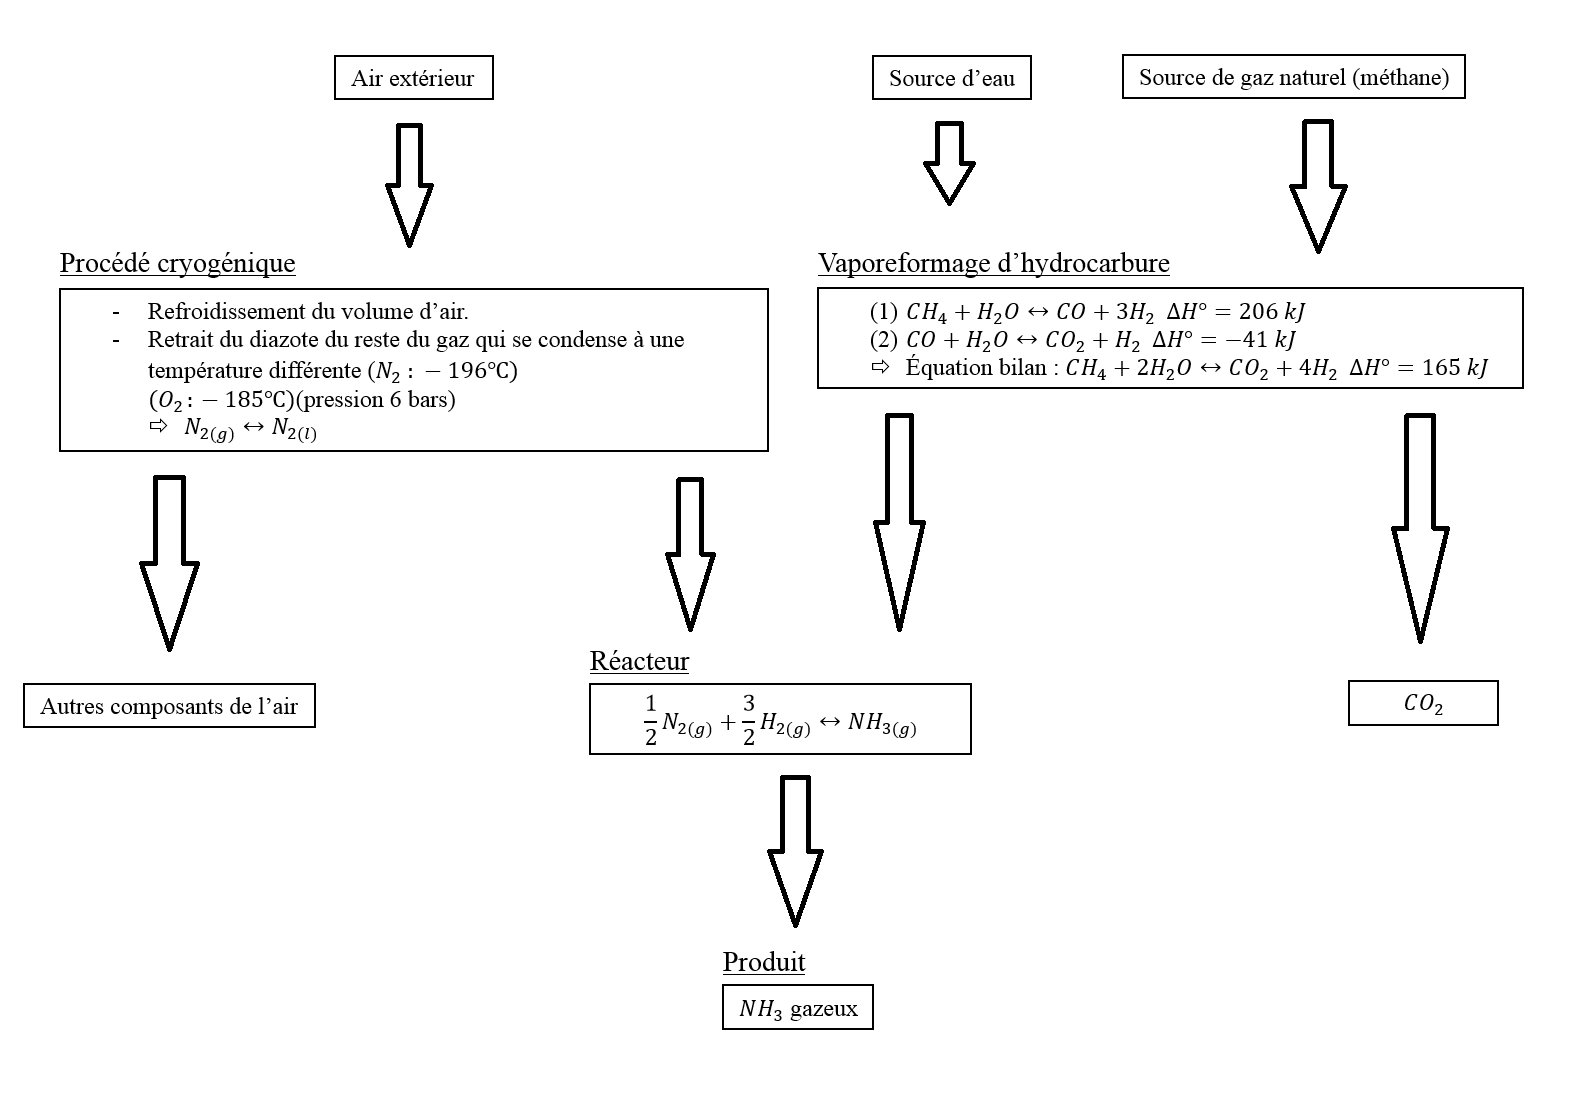
\includegraphics[scale=0.40]{media/flow-sheet.png}}
	\caption{Première ébauche de notre flow-sheet.}
	\label{flow-sheet}
\end{figure}
\newpage

\section{Deuxième version du flow-sheet}
\label{appendix:flow-sheet}
La deuxième version de notre flow-sheet se trouve à la figure \ref{flow-sheet-v2}.

\begin{figure}[htb!]
	\centering
	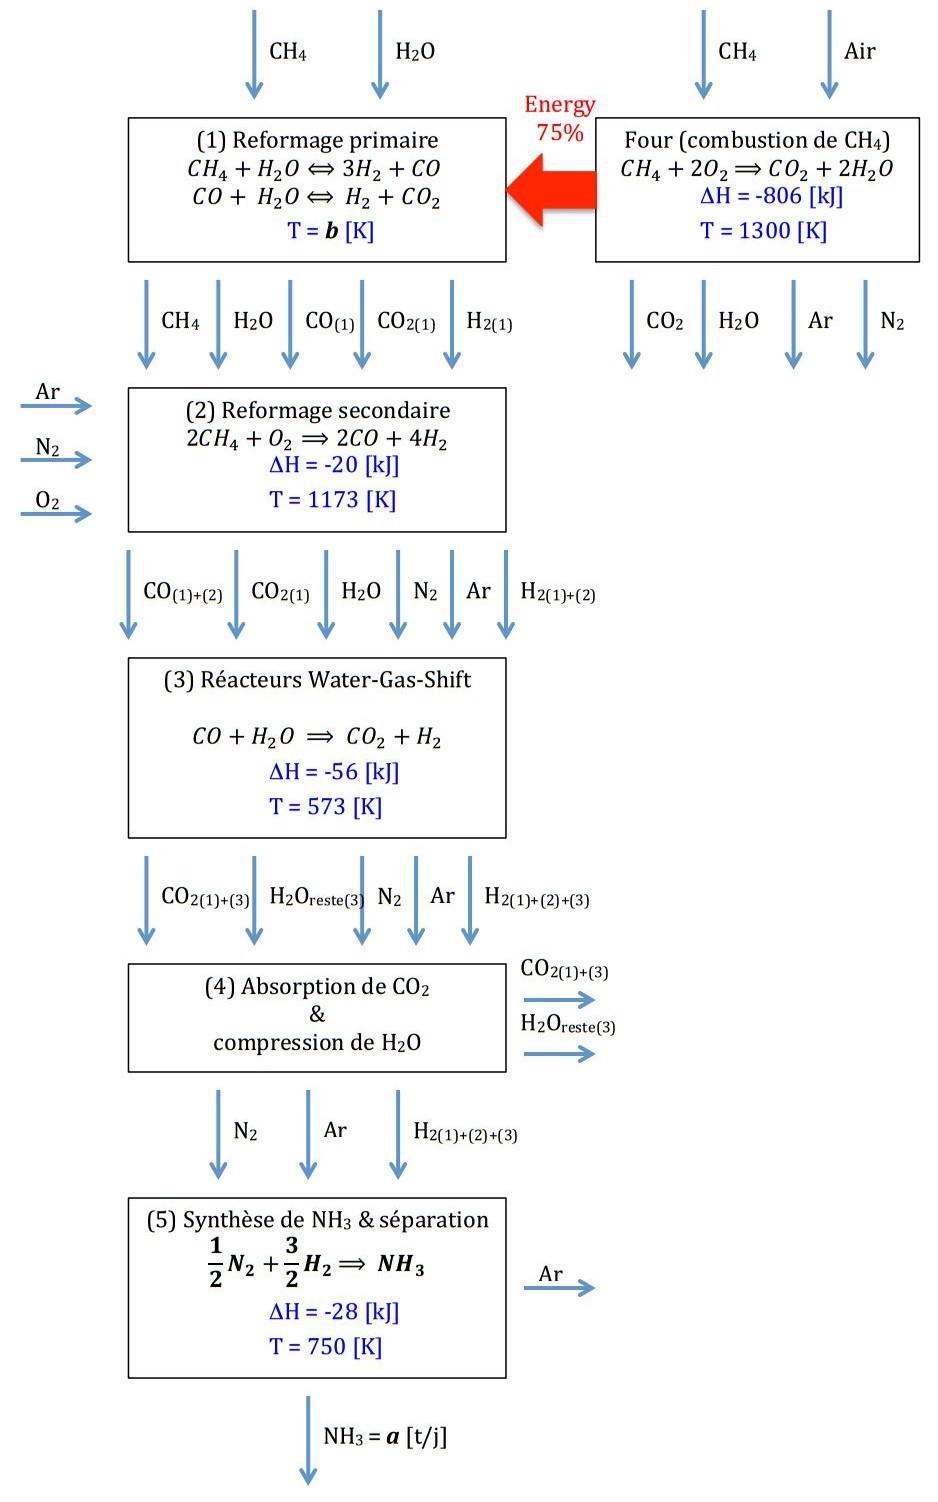
\includegraphics[scale=0.65]{media/flow-sheet-v2.jpg}
	\caption{Deuxième ébauche de notre flow-sheet.}
	\label{flow-sheet-v2}
\end{figure}
\newpage

\section{Code Matlab de l'outil de gestion}
\label{code-matlab-outil}
\lstinputlisting{matlab/OutilDeGestionV2.m}
\lstinputlisting{matlab/ComputeK1.m}
\lstinputlisting{matlab/ComputeK2.m}
\end{document}
